86. $\cfrac{(x-2)(x-3)^2}{x-1}\geqslant x^2-3x\Leftrightarrow \cfrac{(x-2)(x-3)^2-(x-3)x(x-1)}{x-1}\geqslant0\Leftrightarrow$\\
$\cfrac{(x-3)((x-2)(x-3)-x(x-1))}{x-1}\geqslant0\Leftrightarrow\cfrac{(x-3)(x^2-5x+6-x^2+x)}{x-1}\geqslant0
\Leftrightarrow \cfrac{2(x-3)(3-2x)}{x-1}\geqslant0.$ Применив метод интервалов, найдём ответ: $x\in(-\infty;1)\cup\left[\cfrac{3}{2};3\right].$
\begin{figure}[ht!]
\center{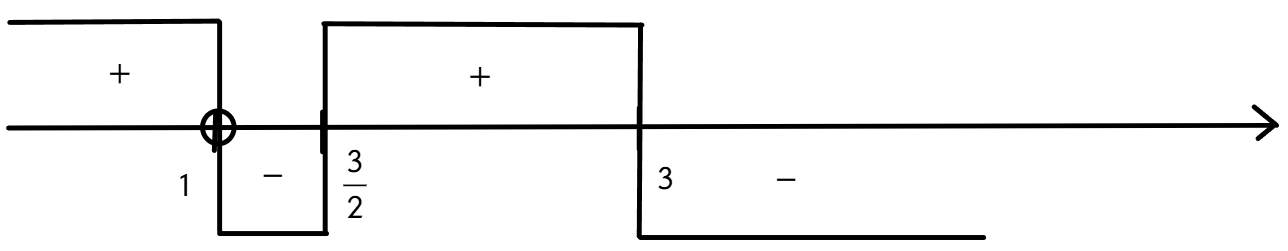
\includegraphics[scale=0.35]{ner9-84.png}}
\end{figure}\\
